%% 電気学会論文誌 公式スタイル v5.0
\documentclass[fleqn]{ieej}
\usepackage[defaultsups]{newtxtext}
\usepackage[varg]{newtxmath}
\usepackage[superscript,nomove]{cite}
\usepackage[dvipdfmx]{graphicx}
\usepackage{booktabs}
\usepackage{url}
\usepackage{algorithm}
\usepackage{algpseudocode}
\renewcommand{\algorithmicrequire}{\textbf{入力:}}
\renewcommand{\algorithmicensure}{\textbf{出力:}}
\usepackage{listings}
\usepackage{xcolor}
\usepackage{placeins}
\lstset{
  basicstyle=\scriptsize\ttfamily,
  breaklines=true,
  frame=single,
  rulecolor=\color{gray!60},
  backgroundcolor=\color{gray!7},
  keywordstyle=\color{blue!70!black}\bfseries,
  commentstyle=\color{green!50!black},
  stringstyle=\color{orange!70!black},
  numbers=none,
  xleftmargin=4pt,
  xrightmargin=4pt,
  aboveskip=4pt,
  belowskip=4pt,
}

%% ── 論文情報 ────────────────────────────────────────────
\FIELD{B}
\YEAR{2026}
\NO{1}
%% 投稿原稿用：全ページのヘッダー・フッター（著作権行・誌名）を非表示
\makeatletter
%% 2ページ以降のランニングヘッド
\def\@evenhead{}\def\@oddhead{}
%% 1ページ目は \thispagestyle{ieej} が呼ばれるので ps@ieej を上書き
\def\ps@ieej{%
  \let\@mkboth\@gobbletwo
  \def\@oddhead{}%
  \def\@evenhead{}%
  \def\@oddfoot{\hfil{\normalfont\thepage}\hfil}%
  \let\@evenfoot\@oddfoot
}
\makeatother

\jtitle{OpenStreetMapに基づくデータ駆動型日本全国送電網モデルの\\自動構築と系統解析}
\etitle{Data-Driven Automated Construction of a Nationwide Japanese\\
        Transmission Grid Model from OpenStreetMap}

\authorlist{%
  \authorentry[lute@u-fukui.ac.jp]{重信 颯人}{Ryuto Shigenobu}{A}{m}
  \authorentry{髙橋 明子}{Akiko Takahashi}{B}{m}
  \authorentry{伊藤 雅一}{Masakazu Ito}{A}{S}
}
\affiliate[A]{福井大学 学術研究院工学系部門 電気・電子工学講座}{%
  Electrical and Electronics Engineering, Faculty of Engineering,
  University of Fukui}
\affiliate[B]{福井大学 学術研究院基盤部門 CN推進本部}{%
  Headquarters for Carbon Neutral Initiatives,
  Faculty of Basic and Generic Researches, University of Fukui}

\begin{document}

%% ── アブストラクト ──────────────────────────────────────
\begin{abstract}
The 2025 Iberian Peninsula blackout highlighted that large-scale grid
failures are difficult to analyse independently when network impedance data
and PMU measurements remain proprietary.
Japan faces the same barrier: bus-level grid models and wide-area
measurement data are not publicly available, impeding reproducible
research on a system undergoing rapid renewable integration
(over 200~GW connected by 2024).
This paper presents \textit{All-Japan-Grid}, an open-source pipeline that
automatically constructs a nationwide transmission grid model from
OpenStreetMap (OSM) crowdsourced data.
A seven-stage attribute completion process reduces 107,383 missing
attributes by 87\%, yielding 6,962 substations, 40,077 lines, and
19,138 plants (274~GW) across all 10 regions of Japan's dual-frequency system.
The pipeline builds sparse bus admittance matrices ($\mathbf{Y}_{\mathrm{bus}}$)
and achieves AC power flow convergence in all 10 regions (previously 0/10).
A MILP unit commitment solver incorporating three-state startup costs
(hot/warm/cold), battery SOC dynamics, and nine inter-regional
interconnection constraints dispatches 783 generators over 24 hours,
revealing a 1.40\% congestion cost premium when all interconnections saturate.
\end{abstract}

\begin{jkeyword}
送電網トポロジ，OpenStreetMap，母線アドミタンス行列，
交流潮流計算，Unit Commitment，オープンデータ
\end{jkeyword}

\begin{ekeyword}
transmission grid topology, OpenStreetMap, bus admittance matrix,
AC power flow, unit commitment, open data
\end{ekeyword}

\maketitle

%% ============================================================
\section{まえがき}

2025年4月，イベリア半島で発生した大規模停電は，
高い再生可能エネルギー比率のもとでの系統慣性不足と
広域連系の脆弱性を改めて世界に示した\cite{entsoe_iberia2025}．
しかし欧州においても，事故後の学術的解析は公開されていない
系統インピーダンスデータや
PMU（位相計測装置）実測値の入手困難が障壁となっており，
独立研究者による再現性のある解析には限界がある．

日本の電力系統においても状況はより深刻である．
10の一般送配電事業者が運用する送電網のインピーダンス・
変圧器特性・バスレベル需要配分は非公開であり\cite{occto2023}，
PMU計測値を含む広域計測システム（WAMS）データも
研究目的で公開されていない．
加えて2012年以降の電力市場自由化に伴い分散型太陽光・風力が
急増し（2024年度末時点で系統接続済み再エネ設備容量は約200~GW），
その系統影響\cite{yokoyama2022,komiyama2012,manabe2013}を定量的に評価する
オープンな基盤がない状態にある．
再エネ事業者・新電力・研究者が電源の系統接続を検討する際には，
空き容量・連系線混雑・潮流変化の定量評価が不可欠であるが，
系統解析に必要なモデルが非公開であるため，独立した事前解析が事実上不可能である．
これは系統解析の「民主化」の欠如であり，接続可能性の判断が
一部事業者に集中し，脆弱箇所の特定や事故原因の独立検証にも
時間と費用を要するという構造的問題を生んでいる．

こうした状況下で，米国はFERC Form~715で
系統モデルを開示し\cite{birchfield2017}，
欧州はENTSO-Eがバスレベルモデルを公開し\cite{entsoe}，
PyPSA-Eur等のオープンモデルが再エネシナリオ分析や
脆弱性評価に活用されている\cite{pypsa_eur}．
一方，日本全国の送電網を対象とした
バスレベルのオープンデータセットは著者らの知る限り存在しない．

本研究は，クラウドソーシング地理情報データベース
OSM\cite{osm}から日本全国の送電網トポロジを自動抽出し，
多段階属性補完と合成電気パラメータ付与により
オープン基盤データセットを自動構築する
パイプライン\textit{All-Japan-Grid}を開発した
（図\ref{fig:map}）．
系統解析そのものを目的とするのではなく，
OSM由来データが潮流計算・UC・動揺解析の各手法に
接続可能かを検証する予備的試算として位置付けられる．

主な貢献：
\begin{enumerate}
  \item 全国10地域・6,962バス・40,077送電線のオープンデータセット
  \item 7段階属性補完による欠損87\%削減
  \item 疎$\mathbf{Y}_{\mathrm{bus}}$自動構築と全地域AC潮流収束の達成
  \item 783機・3状態起動コスト・蓄電池SOCを含むMILP UCの求解
  \item イベリア停電型の過渡安定・N-$x$解析の実施
\end{enumerate}

\begin{figure}[t]
  \centering
  
\includegraphics[width=\columnwidth]{figs/fig_national_all.png}
  \caption{全国送電網トポロジ（OSM由来，電圧クラス別色分け）\\
  {\small 赤：500~kV，橙：275~kV，黄：154~kV，緑：110~kV，青：66~kV}}
  \label{fig:map}
\end{figure}

PyPSA-Eur\cite{pypsa_eur}，SciGRID\cite{medjroubi2017}，
Arderne ら\cite{arderne2020}のグローバルマッピング，
PyPSA\cite{brown2018pypsa}等はENTSO-E・OSMから欧州・世界の系統モデルを自動構築した先行事例であるが，
日本全国の送電系統を対象としたオープンデータセットは著者らの知る限り存在せず，本研究はその空白を埋める最初の試みである．

%% ============================================================
\section{全国送電網モデル自動構築パイプライン}

パイプライン全体の流れをAlgorithm~\ref{alg:pipeline}に示す．
OSMから地理データを取得し，7段階属性補完とトポロジ再構築を
経て，pandapowerモデルおよび疎$\mathbf{Y}_{\mathrm{bus}}$を構築する．

\begin{algorithm}[t]
\caption{All-Japan-Grid 系統構築・解析パイプライン}
\label{alg:pipeline}
\begin{algorithmic}[1]
\Require 地域リスト $\mathcal{R}$，最大距離閾値 $d_\text{max}=50$~km
\Ensure pandapowerモデル，$\mathbf{Y}_\text{bus}$，UC結果，動揺解析結果
\For{各地域 $r \in \mathcal{R}$}
  \State \textbf{[取得]} Overpass APIタイル分割クエリ（OSM ID重複除去）
  \State \textbf{[補完]} 7段階属性補完（Nominatim・P03照合・燃料正規化）
  \State \textbf{[トポロジ]} 送電線端点 $\to$ 最近傍変電所 Haversine距離マッチング
  \State \textbf{[電圧]} 日本標準値（66, 110, 154, 275, 500 kV）へスナップ
  \State \textbf{[変圧器]} 電圧比$\geq 1.5$の接続を変圧器として自動挿入
  \State \textbf{[連結]} KD木で孤立成分を補修（補修後連結率99.7\%）
  \State \textbf{[パラメータ]} 電圧クラス別 $(R,X,B,I_\text{max})$ 参照テーブル付与
  \State \textbf{[モデル化]} pandapowerネットワーク構築
  \State \textbf{[$\mathbf{Y}_\text{bus}$]} PYPOWER内部変換で疎CSC行列を構築
\EndFor
\State \textbf{[AC潮流]} 20手法チェーン（NR $\to$ GS $\to$ FDPF-BX $\to$ \ldots）
\State \textbf{[UC]} MILP（PuLP+HiGHS）: $\min\sum_{g,t}[C_f^g p_{g,t}+C_{\mathrm{NL}}^g u_{g,t}+C_{\mathrm{SU}}^g v_{g,t}+C_{\mathrm{SD}}^g w_{g,t}]$
\State \textbf{[動揺]} Kron縮約 $\to$ RK45: $\tfrac{2H_i}{\omega_s}\ddot{\delta}_i = P_{m,i}-P_{e,i}-D_i\dot{\delta}_i$，N-$x$解析
\State \textbf{[モード]} 固有値解析: $\lambda_k=\sigma_k\pm j\omega_{d,k}$
\end{algorithmic}
\end{algorithm}

\subsection{OSMデータ取得と属性補完}

\paragraph{取得対象と生データの品質}
変電所（\texttt{power=substation}），送電線（\texttt{power=line/cable}），
発電所（\texttt{power=plant}）をOverpass~API\cite{overpass}で取得する．
OSMはボランティアによるクラウドソーシングデータであり，
生データの品質は地域・設備種別によって大きく異なる（表~\ref{tab:osm_attr}）．
特に電圧属性については，
「\texttt{voltage=0}」「\texttt{voltage=}空文字」「単位系混在（V/kV）」等の
不正値を含む線路が全体の約30\%に存在し，そのままでは系統解析に使用できない．
発電所の設備容量（\texttt{capacity\_mw}）は太陽光を中心に約93\%が未記録である．

\begin{table}[t]
  \caption{OSMから取得できる属性と記録状況（全国集計）}
  \label{tab:osm_attr}
  \centering\small
  \begin{tabular}{llcc}
    \toprule
    属性 & OSMタグ & 生記録率 & 補完後 \\
    \midrule
    \multicolumn{4}{l}{\textit{位置情報}}\\
    地理座標 & \texttt{geometry} & $\approx$100\% & 100\% \\
    変電所輪郭 & polygon & $\approx$60\% & centroid補完 \\
    \multicolumn{4}{l}{\textit{電気属性}}\\
    電圧（正常値） & \texttt{voltage} & $\approx$70\% & $\approx$85\%† \\
    架空/地中区分 & \texttt{location} & $\approx$30\% & \textit{未補完}\\
    ケーブル数 & \texttt{cables} & $\approx$40\% & \textit{未補完}\\
    インピーダンス & — & 0\% & 電圧別参照表 \\
    変圧器特性 & — & 0\% & 電圧比推定 \\
    \multicolumn{4}{l}{\textit{設備情報}}\\
    事業者名 & \texttt{operator} & $\approx$65\% & $\approx$100\% \\
    発電燃料種 & \texttt{plant:source} & $\approx$85\% & $\approx$100\% \\
    設備容量 & \texttt{capacity\_mw} & $\approx$7\%†† & P03照合で補完 \\
    \multicolumn{4}{l}{\textit{系統情報（OCCTOで代替）}}\\
    連系線容量 & — & 0\% & OCCTO公開値 \\
    需要量 & — & 0\% & 電圧比例推定 \\
    混雑・市場価格 & — & 0\% & OCCTO市場データ \\
    遮断器情報 & — & 0\% & \textit{非公開・未補完} \\
    \bottomrule
    \multicolumn{4}{l}{†電圧クラス（66/110/154/275/500~kV）へのスナップ後}\\
    \multicolumn{4}{l}{††大型電源のみ。太陽光（17,527箇所）のほぼ全てが未記録}\\
  \end{tabular}
\end{table}

生データには名称欠損49,384件，事業者欠損41,563件，
燃料種別未知334件を含む107,383件の属性欠損が存在した．
表~\ref{tab:enrich}に示す7段階パイプラインで87\%（93,297件）を補完した．

\begin{table}[t]
  \caption{7段階属性補完パイプライン}
  \label{tab:enrich}
  \centering\small
  \begin{tabular}{clc}
    \toprule
    段階 & 手法 & 主対象 \\
    \midrule
    1 & ベースライン監査・欠損分類 & 全体 \\
    2 & Nominatim逆ジオコーディング & 変電所名 \\
    3 & MLIT P03施設データ空間照合 & 発電所 \\
    4 & Overpassタグ一括取得（500件/回） & 属性全般 \\
    5 & Nominatimジオコーディング（後退） & 発電所 \\
    6 & 最近傍変電所マッチング（50~km閾値） & 送電線名 \\
    7 & 燃料種別正規化（44エントリ対応表） & 発電所 \\
    \bottomrule
  \end{tabular}
\end{table}

\paragraph{GeoJSONデータ形式}
取得・補完後の全データはGeoJSON形式（RFC~7946準拠，Listing~1）で
\texttt{\{region\}\_\{substations|lines|plants\}.geojson}の30ファイルとして管理する．

\begin{figure}[h]
\begin{lstlisting}[language={}]
{"type":"FeatureCollection","features":[
  {"type":"Feature",
   "geometry":{"type":"Point",
     "coordinates":[135.66,35.54]},
   "properties":{
     "name":"嶺南変電所",
     "voltage":"500000",
     "operator":"関西電力",
     "osm_id":123456789,
     "_enriched_by":"p03_match"}}]}
\end{lstlisting}
\vspace{-6pt}
{\scriptsize Listing~1: 変電所GeoJSONフィーチャの例（抜粋）}
\end{figure}

\paragraph{Overpass APIクエリとCLIコマンド}
各地域を緯度経度$N\times M$タイルに分割し，各タイルに対して
以下のOverpass~QL（Overpass Query Language）を発行する：

\begin{lstlisting}[language={}]
[out:json][timeout:300][bbox:35.0,138.5,37.0,141.0];
(node["power"="substation"]; way["power"="substation"];
 way["power"="line"]; way["power"="cable"];
 node["power"="plant"]; way["power"="plant"];
 relation["power"="plant"];);
out body;>;out skel qt;
\end{lstlisting}

OSM~IDによる境界重複除去後，各レイヤをGeoJSON形式で保存する．
全国10地域の取得・属性補完所要時間は約2時間である．

なお，OCCTO\cite{occto2023}が公開する9連系線の断面容量はUCモデルのフロー上限として利用した．
バスレベルのインピーダンス・需要・遮断器情報はOSM・OCCTOいずれにも存在せず，合成推定値で代替する（表\ref{tab:osm_attr}参照）．

\subsection{地理トポロジ再構築}

OSM送電線は座標点列のみを持つため，Haversine距離で各端点に
最近傍変電所を対応付ける（閾値$d_{\mathrm{max}}=50$~km）：
\begin{equation}
  d = 2R\arctan2\!\bigl(\sqrt{a},\sqrt{1-a}\bigr)
  \label{eq:haversine}
\end{equation}
ここで$a = \sin^2(\Delta\phi/2)+\cos\phi_1\cos\phi_2\sin^2(\Delta\lambda/2)$，
$R=6{,}371$~kmである．

電圧比1.5倍超の接続は変圧器として解釈し，電圧クラス別デフォルト
パラメータ（$S_n$，$v_k$，$v_{kr}$）を付与する．
KD木による最近傍探索で孤立成分を主成分に接続し（補修後連結率99.7\%），
全地域で一貫したトポロジを確保する．

Fig.~\ref{fig:regional}に各地域の詳細ネットワークを，
Fig.~\ref{fig:satellite}に衛星画像との位置照合結果を示す．

\begin{figure*}[t]
  \centering
  
\includegraphics[width=\textwidth]{figs/fig_regional_networks.png}
  \caption{各地域送電網トポロジ（全10地域，電圧クラス別色分け）}
  \label{fig:regional}
\end{figure*}
さらにFig.~\ref{fig:layers}に3種のGeoJSONレイヤを
独立に展開した全国可視化を示す：
(a)~送電線ネットワークのみ（40,077本），
(b)~変電所のみ（6,962箇所，電圧クラス別），
(c)~発電所の大型集中電源と分散型再エネの2分類（計19,138箇所）．
特に(c)において太陽光・風力を主体とする分散型再エネが
関東・東海・九州北部の日射良好地帯に面的に展開する様子が明確に現れている．

\begin{figure*}[t]
  \centering
  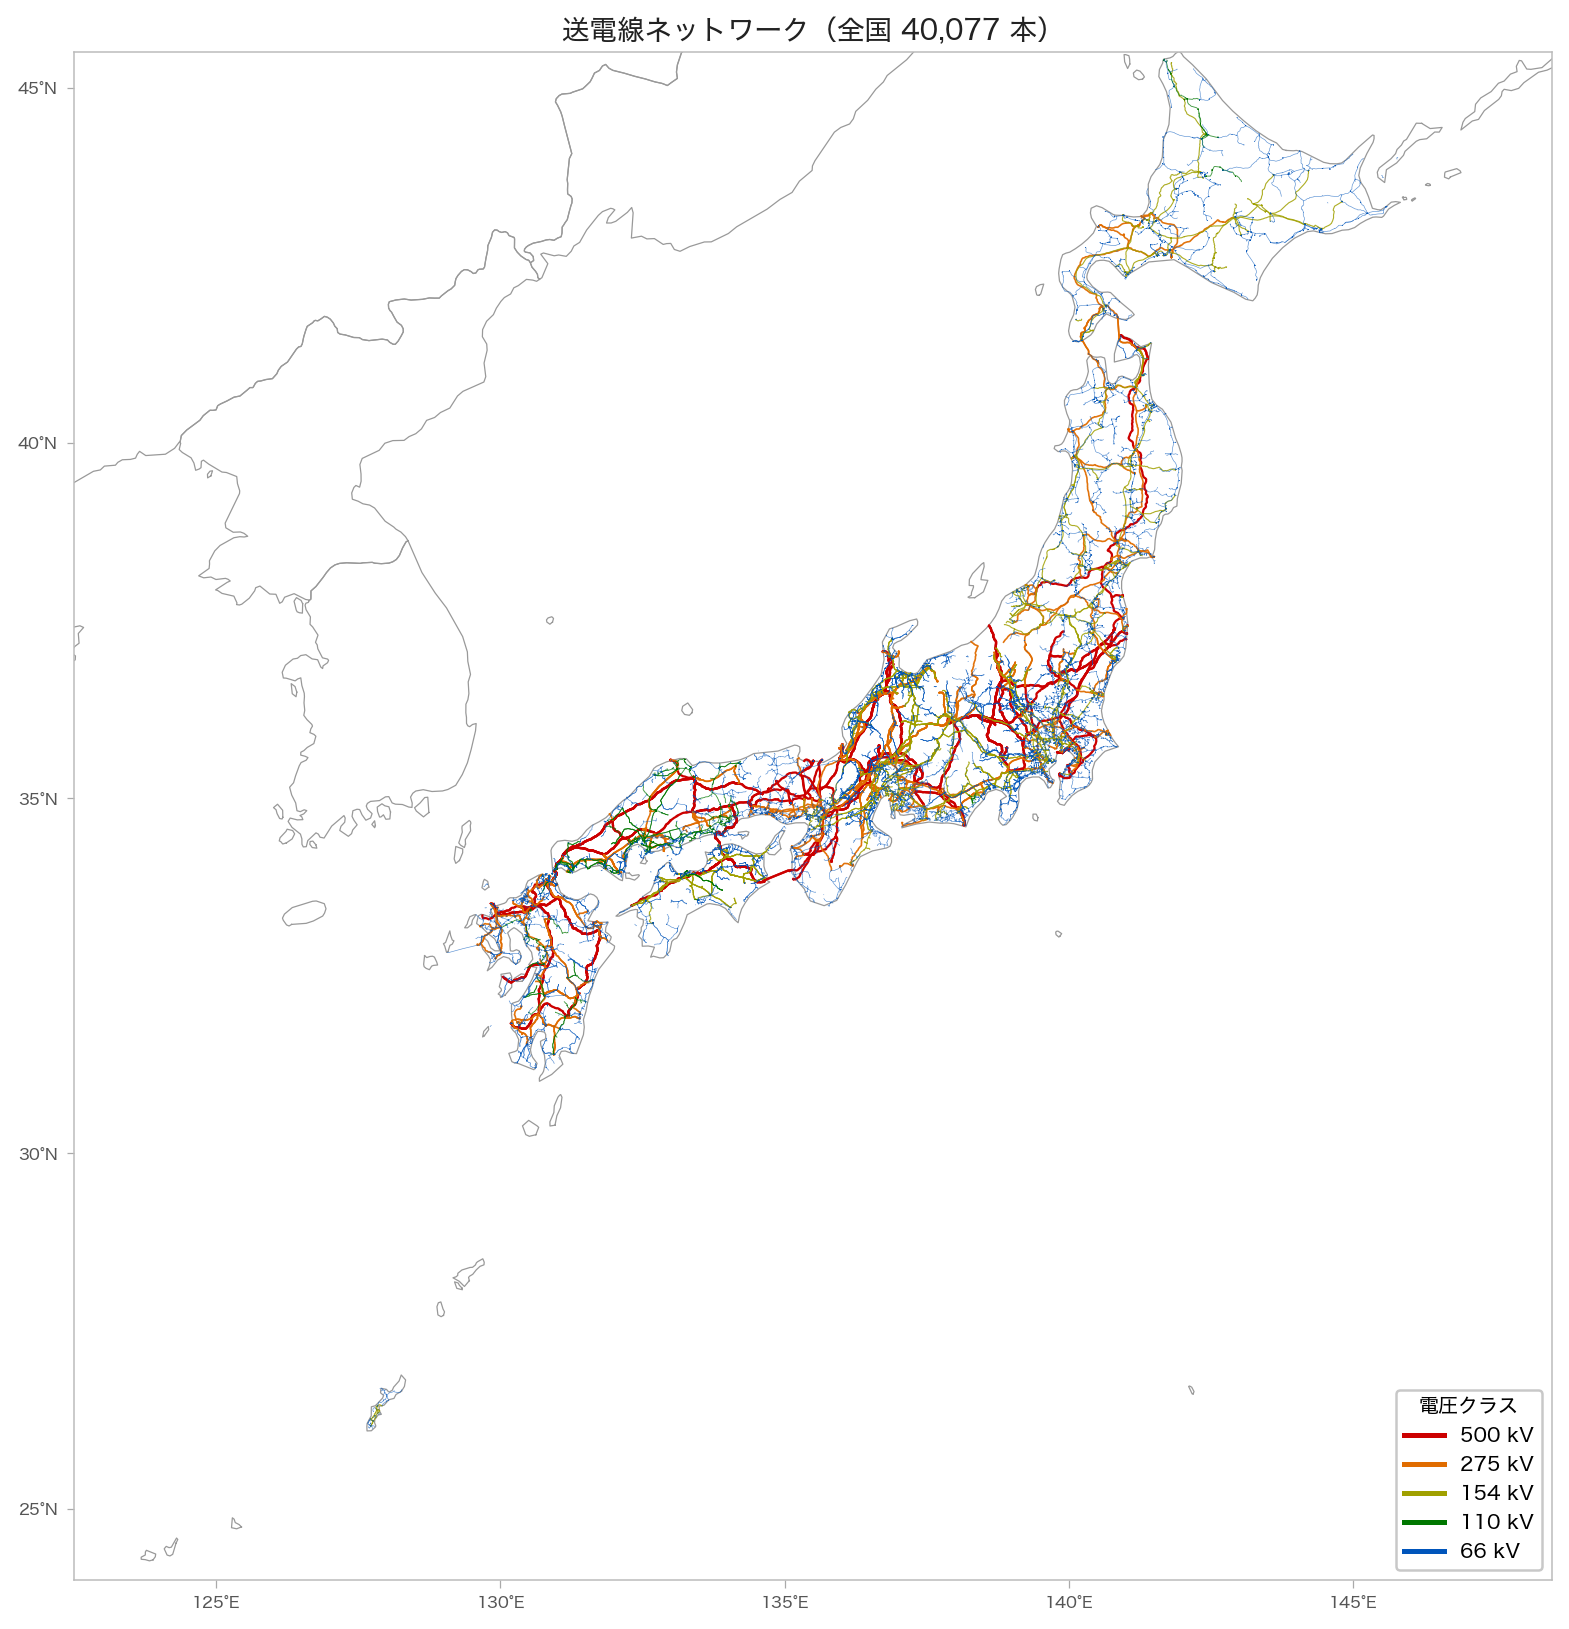
\includegraphics[width=0.325\textwidth]{figs/fig_layer_network.png}%
  \hfill
  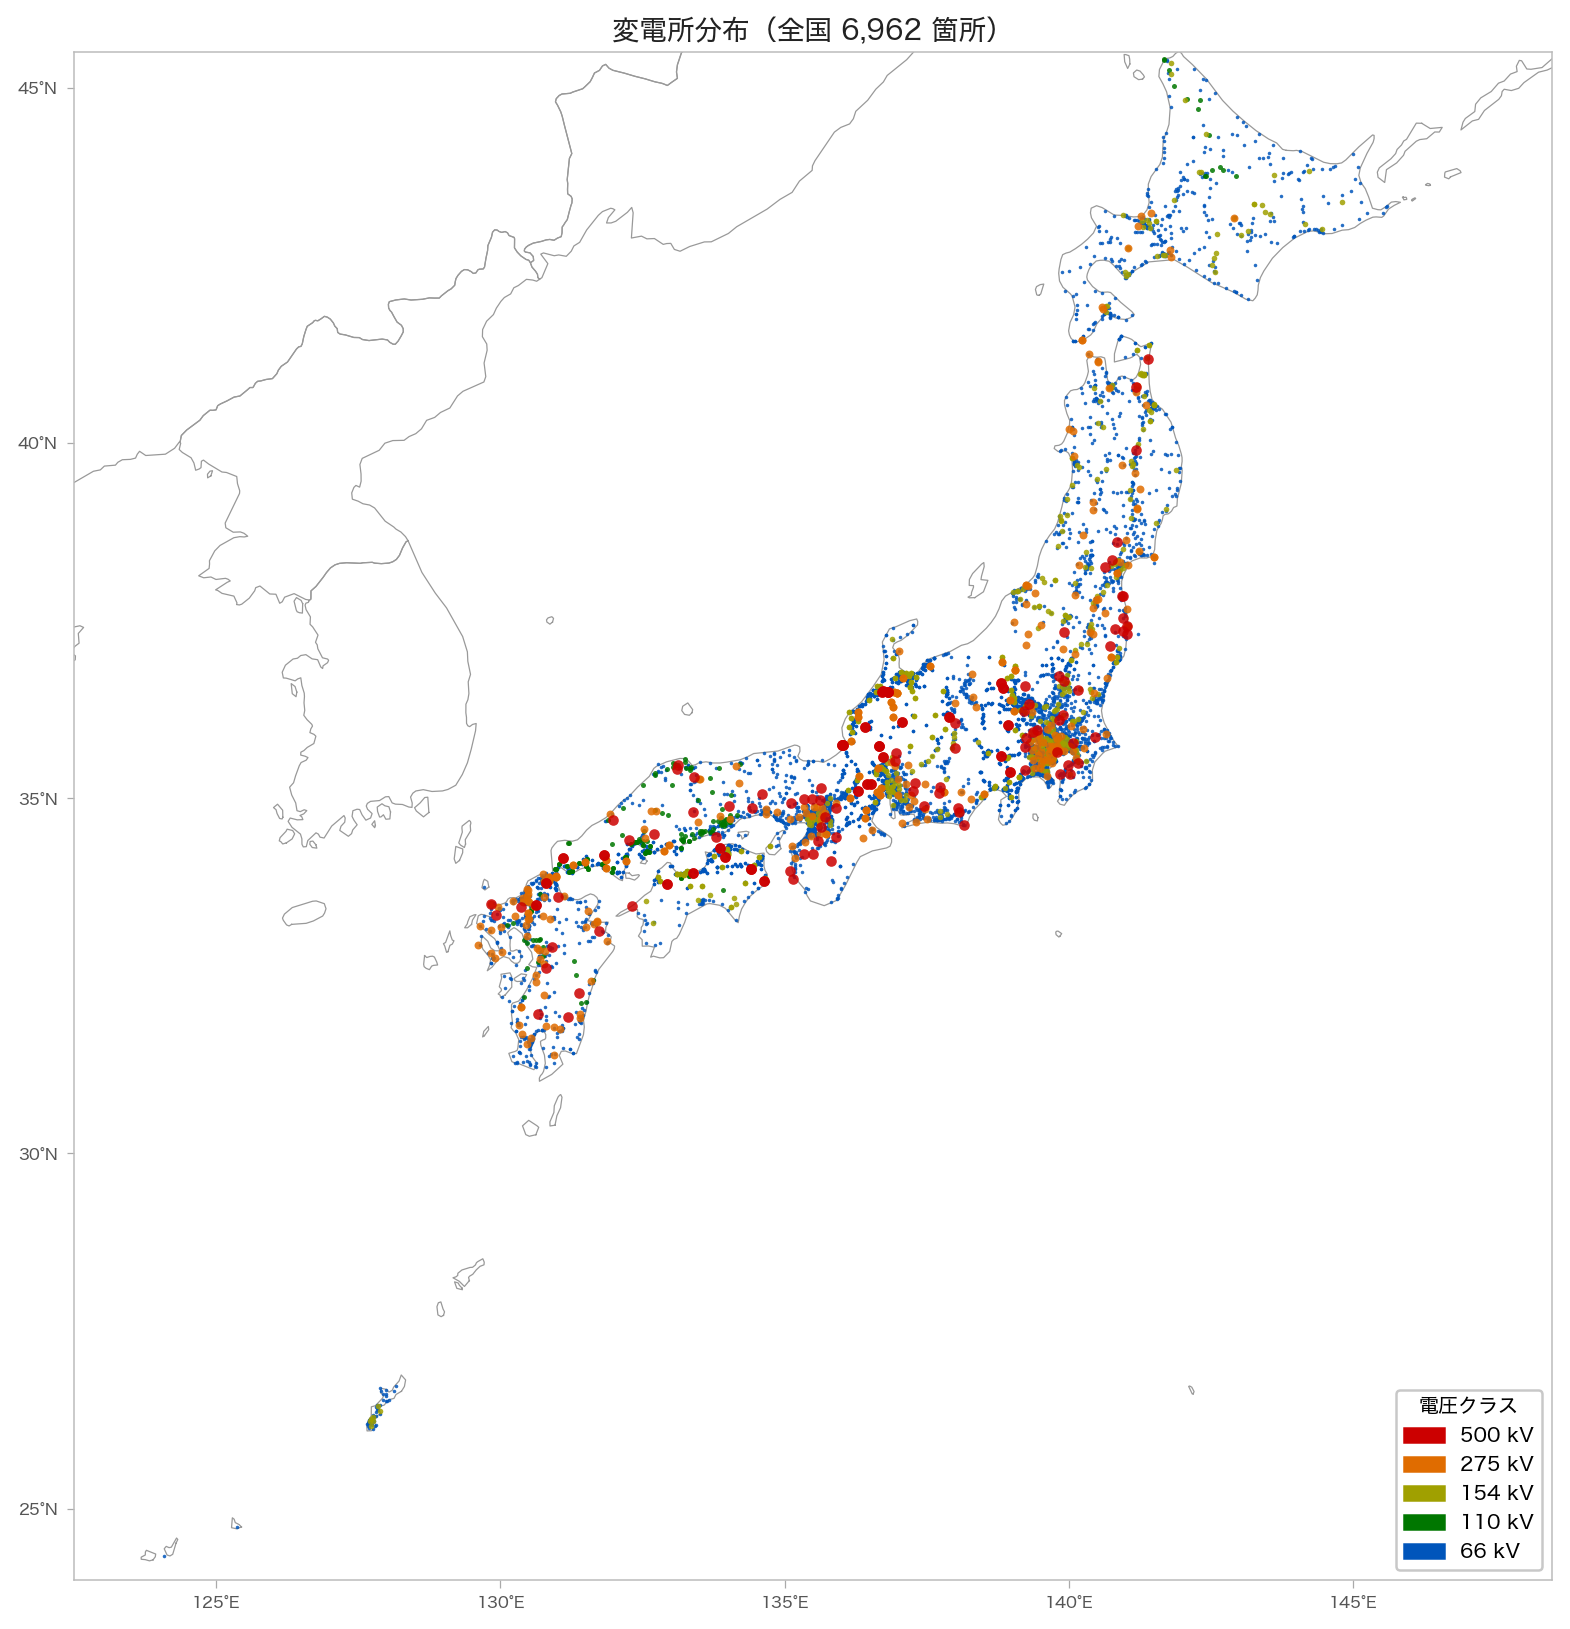
\includegraphics[width=0.325\textwidth]{figs/fig_layer_substations.png}%
  \hfill
  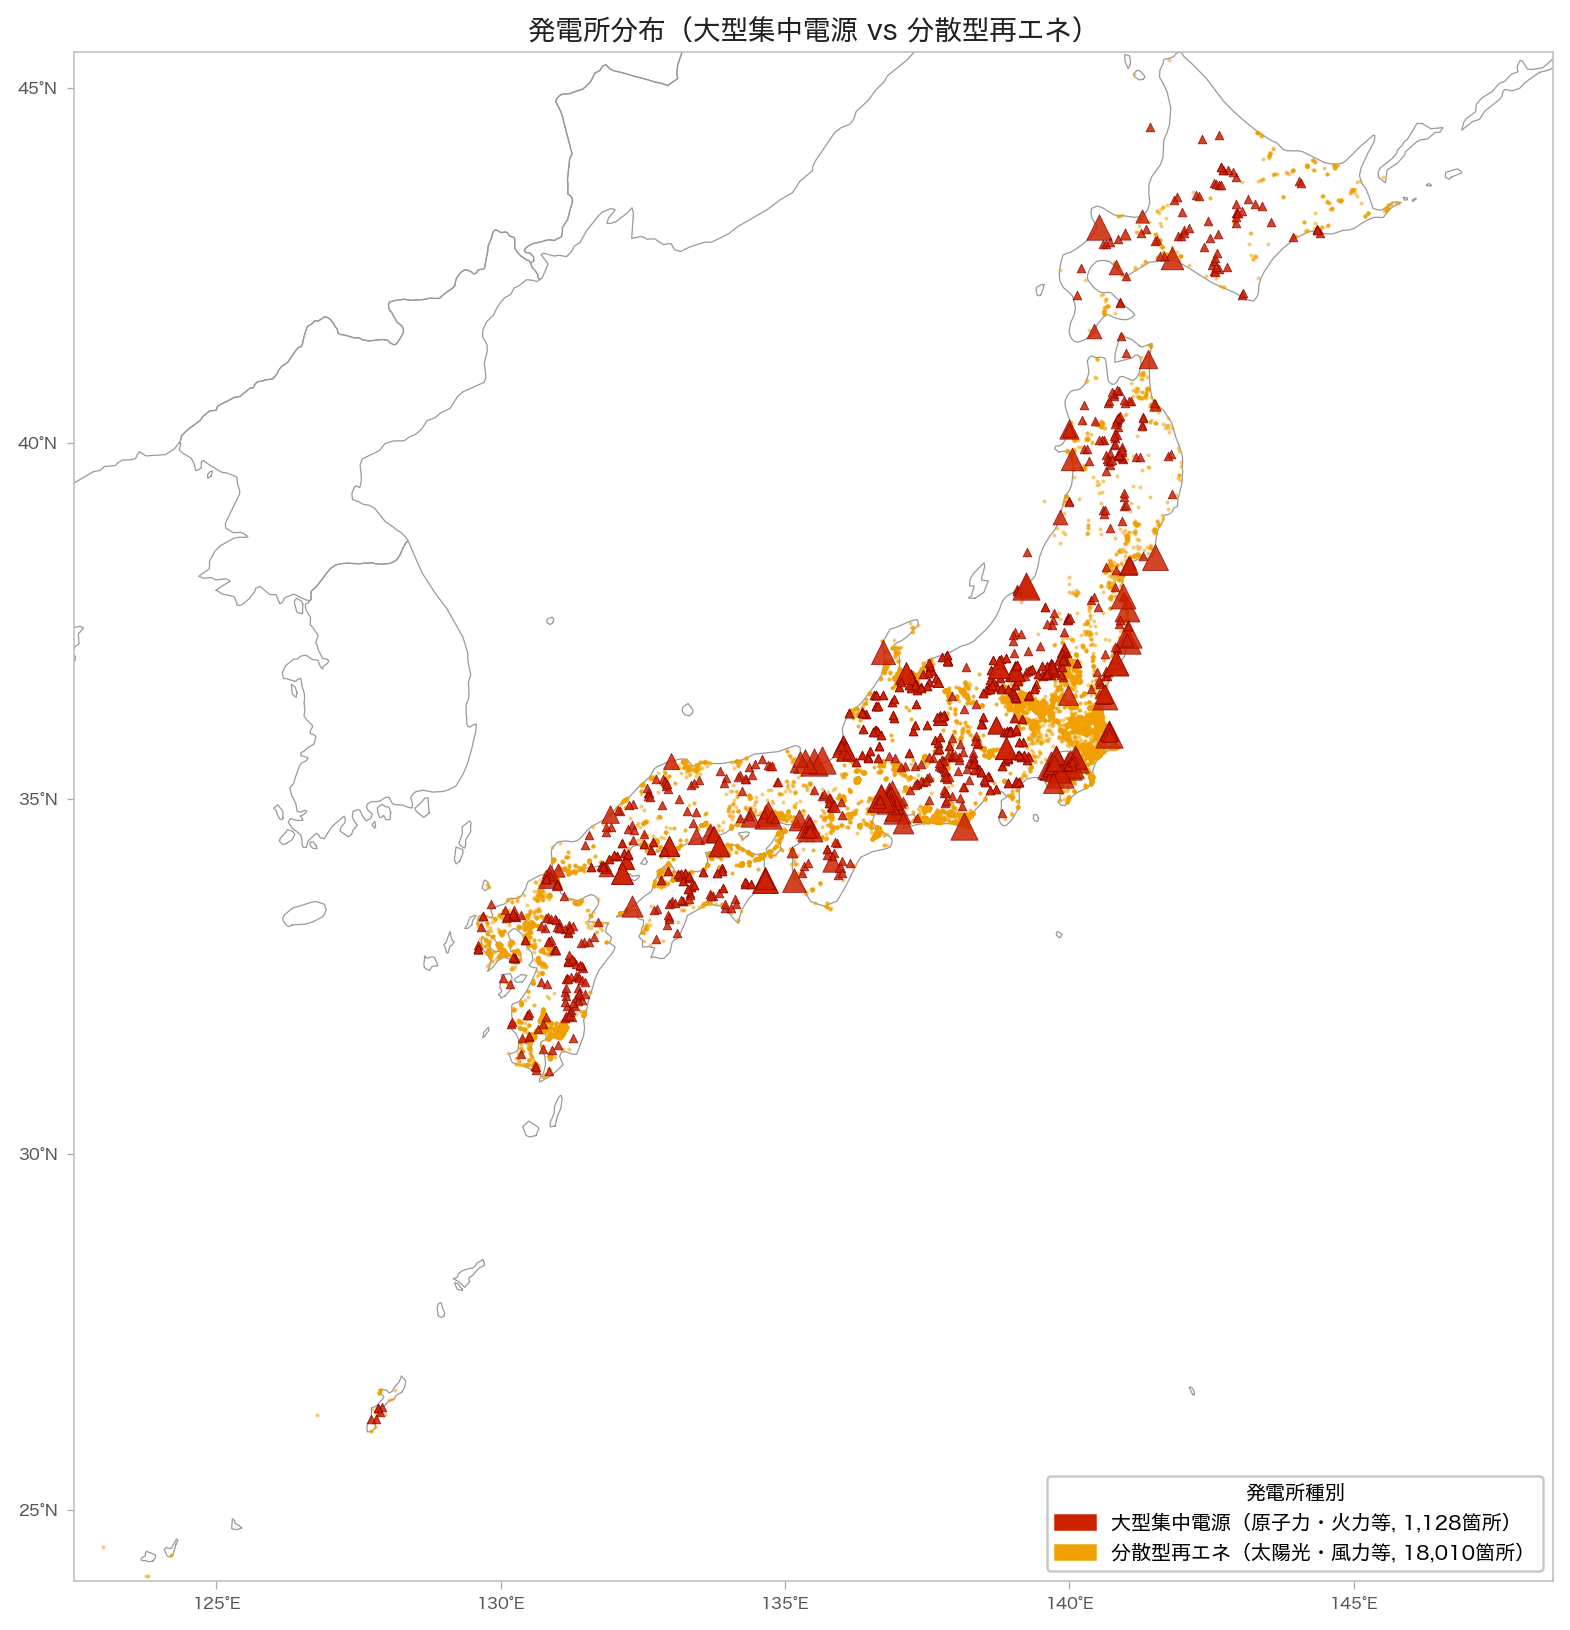
\includegraphics[width=0.325\textwidth]{figs/fig_layer_plants.png}
  \caption{GeoJSONレイヤ別展開：
  (a)~送電線ネットワーク（40,077本，電圧クラス別色分け），
  (b)~変電所分布（6,962箇所），
  (c)~発電所分類（赤△：大型集中電源[原子力・火力・大型水力等, 659箇所]，
  黄●：分散型再エネ[太陽光・風力等, 18,479箇所]）}
  \label{fig:layers}
\end{figure*}

\begin{figure*}[t]
  \centering
  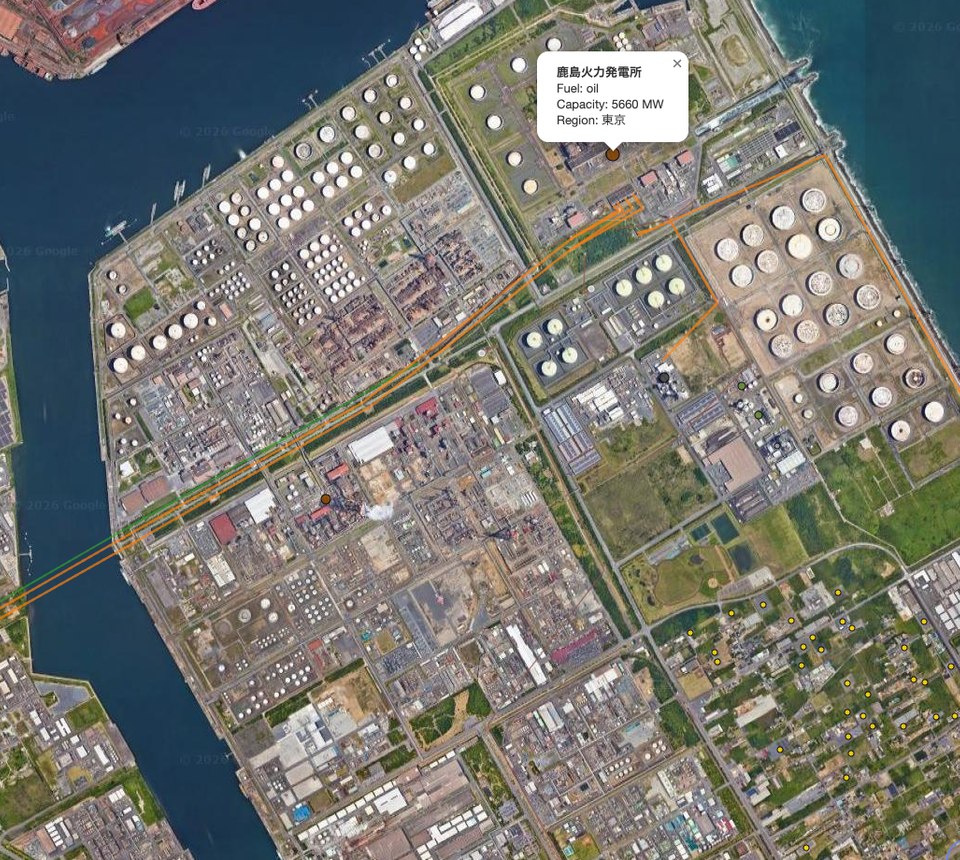
\includegraphics[width=0.325\textwidth]{figs/sat_kashima.png}\hfill
  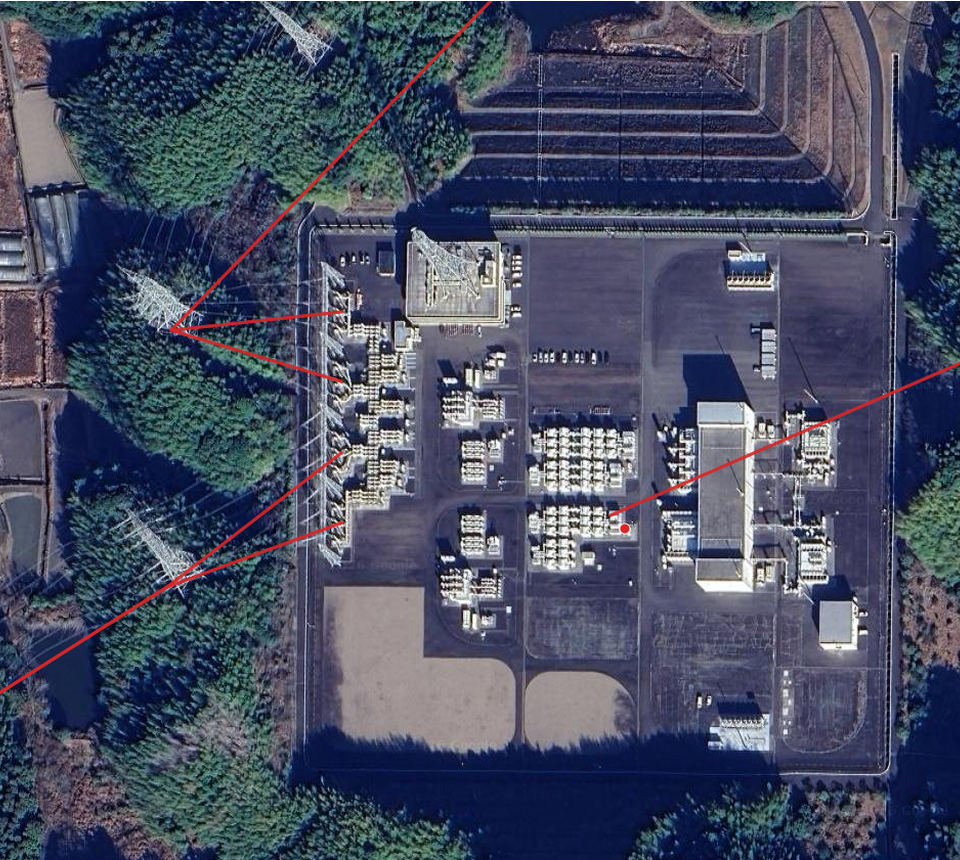
\includegraphics[width=0.325\textwidth]{figs/sat_anan_fc.png}\hfill
  
\includegraphics[width=0.325\textwidth]{figs/sat_reinan.png}
  \caption{衛星画像との重畳照合による位置精度確認：
  (左)~鹿島火力発電所（茨城県）——右下に大規模太陽光エリア，
  本体発電所から伸びる 500~kV 送電線が視認可能；
  (中)~阿南周波数変換所（徳島県）——変換所施設と
  東西連系 DC 300~MW の引込み線が明確；
  (右)~嶺南変電所（福井県）——若狭湾原子力集積地帯に位置する
  500~kV 基幹変電所で複数の超高圧回線が集約される様子を確認}
  \label{fig:satellite}
\end{figure*}

\subsection{電気パラメータ付与と$\mathbf{Y}_{\mathrm{bus}}$構築}

OSMは電気的パラメータを持たないため，OCCTO設計資料および
文献値\cite{glover}に基づく電圧クラス別参照テーブルから
$R$，$X$，$B$，$I_{\mathrm{max}}$を付与する（表\ref{tab:params}）．

\begin{table}[t]
  \caption{電圧クラス別送電線パラメータ}
  \label{tab:params}
  \centering\small
  \begin{tabular}{lrrrr}
    \toprule
    $V$ (kV) & $R$ ($\Omega$/km) & $X$ ($\Omega$/km) & $B$ ($\mu$S/km) & $I_{\max}$ (kA) \\
    \midrule
    500 & 0.012 & 0.290 & 4.10 & 4.0 \\
    275 & 0.028 & 0.325 & 3.85 & 2.0 \\
    154 & 0.050 & 0.380 & 3.50 & 1.0 \\
    110 & 0.055 & 0.385 & 3.45 & 0.9 \\
     66 & 0.120 & 0.400 & 3.20 & 0.6 \\
    \bottomrule
  \end{tabular}
\end{table}

pandapower\cite{pandapower}によりバス・送電線・発電機・変圧器を登録後，
内部PYPOWER変換を通じて疎母線アドミタンス行列を構築する：
\begin{equation}
  Y_{ij}=\begin{cases}
    \displaystyle\sum_{k}y_{ik}+\sum_k\tfrac{jB_{ik}}{2} & (i=j)\\[4pt]
    -y_{ij} & (i\neq j)
  \end{cases}
  \label{eq:ybus}
\end{equation}
ここで$y_{ij}=(R_{ij}+jX_{ij})^{-1}$はブランチアドミタンスである．
$\mathbf{Y}_{\mathrm{bus}}$はCSC疎行列形式で保持し（充填率$<0.01$\%），
LU分解による効率的な潮流計算を実現する．
Fig.~\ref{fig:ybus}に全国統合$\mathbf{Y}_{\mathrm{bus}}$のブロック対角構造を示す．

\begin{figure*}[t]
  \centering
  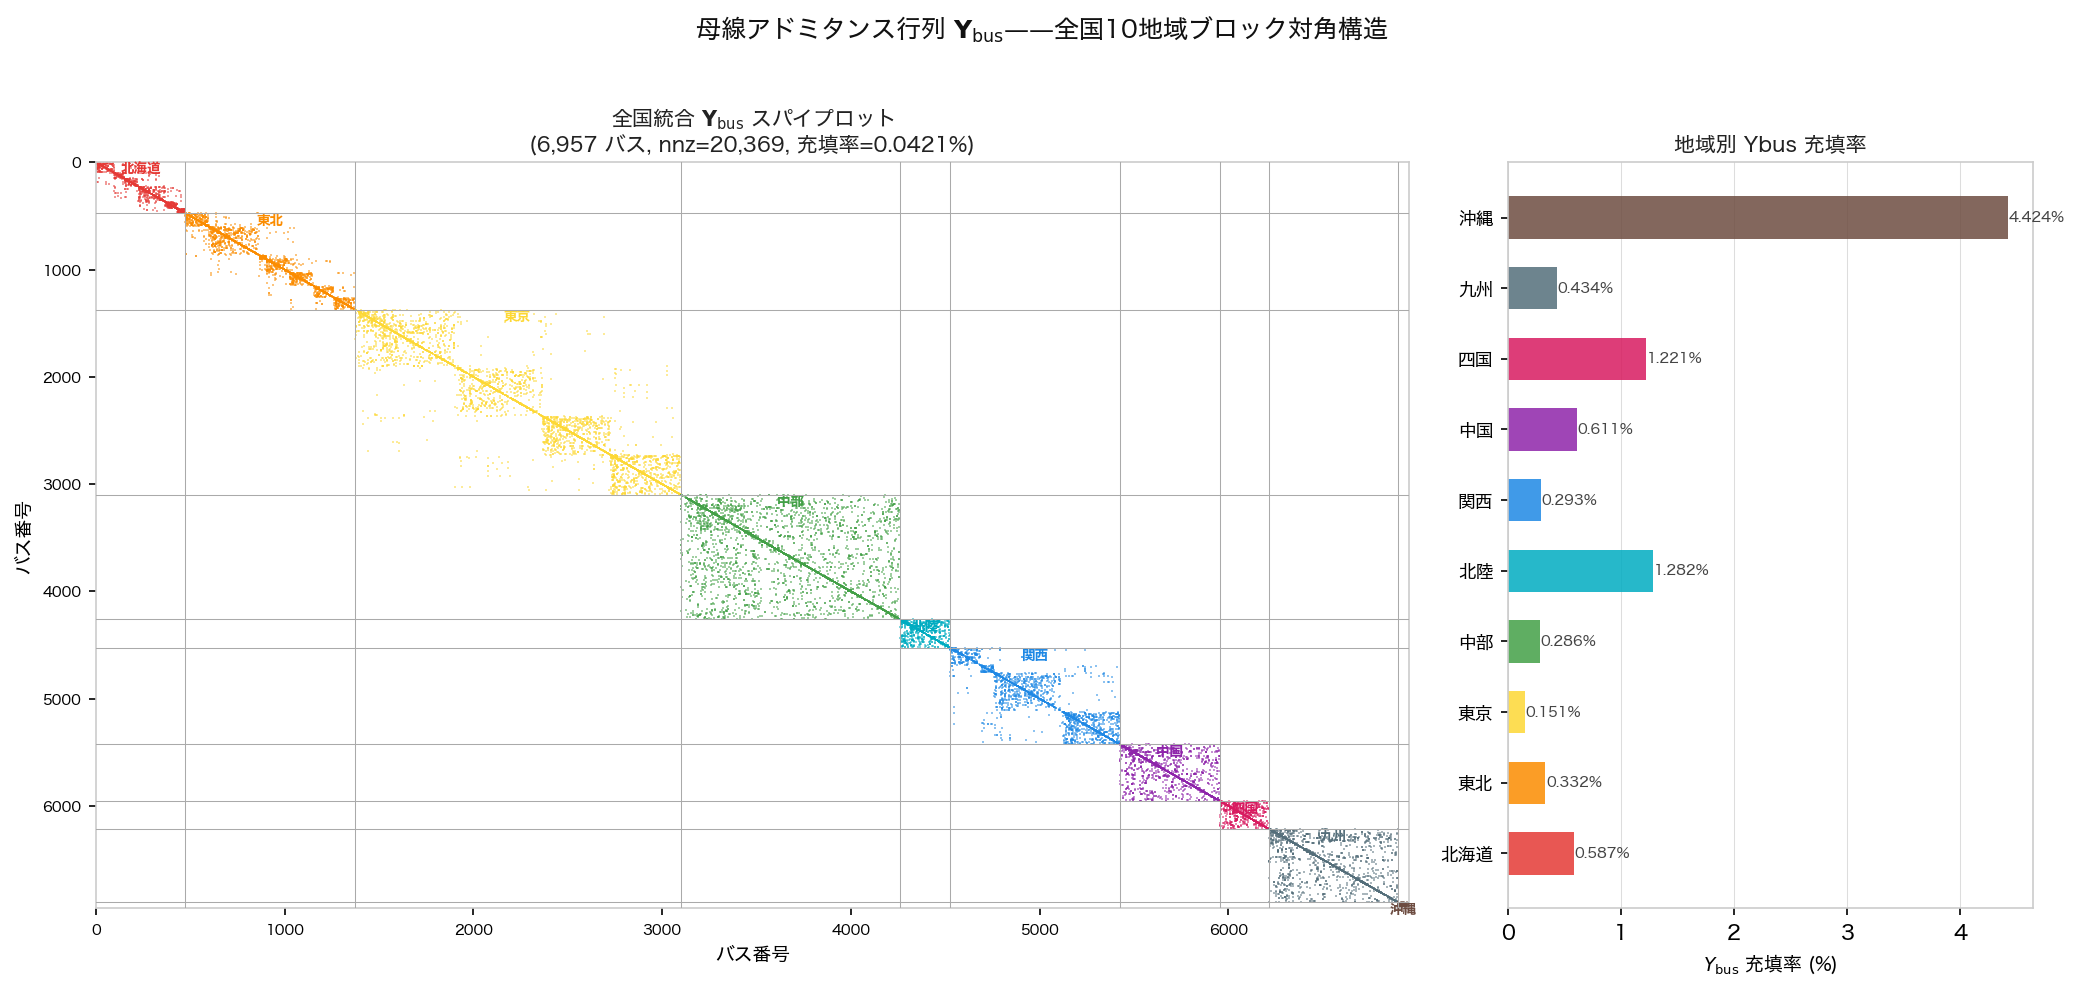
\includegraphics[width=\textwidth]{figs/fig_ybus_national.png}
  \caption{全国統合$\mathbf{Y}_{\mathrm{bus}}$（6,962バス，20,369非零要素，充填率$<$0.01\%）——
  ブロック対角構造（10地域独立）を確認；右グラフは地域別充填率（東京・東北が最大）}
  \label{fig:ybus}
\end{figure*}

\subsection{AC潮流ソルバ（20手法）と収束検証}

$(\mathbf{Y}_{\mathrm{bus}},\mathbf{S}_{\mathrm{bus}},\mathbf{V}_0,
\mathrm{ref,pv,pq})$を共通引数とする統一APIで4カテゴリ20手法を実装した：
pandapowerラッパ5種（NR，GS，FDPF-BX/XBほか），
カスタムNewton-Raphson 7種（岩本法，LM法ほか），
反復法4種（SOR，加速GSほか），デカップル法4種（FDPF，続行PFほか）\cite{zimmerman2011}．
NR法\cite{tinney1967}および高速分離潮流法\cite{stott1974}はいずれも
IEEE 14/118/300-busで全手法の収束を確認済みである．
標準NR法の更新式：
\begin{equation}
  \mathbf{J}
  \begin{bmatrix}\Delta\theta\\\Delta|V|/|V|\end{bmatrix}
  =\begin{bmatrix}\Delta P\\\Delta Q\end{bmatrix},\quad
  \|\Delta\mathbf{S}\|_\infty<10^{-8}
  \label{eq:nr}
\end{equation}

パイプライン整備前はAC収束が0/10であったが，
発電機15,980台の自動登録，電圧零バスの補完推定，
変圧器3,956台の自動挿入，スラックバス最適選択（500/275~kV優先）に
より全10地域で収束を達成した（表\ref{tab:pf}）．
東京地域の損失994~MWは全損失の62\%を占め，
44~GW超の大規模負荷を反映する．


\begin{table}[t]
  \caption{全地域AC潮流計算結果}
  \label{tab:pf}
  \centering\small
  \begin{tabular}{lrrrr}
    \toprule
    地域 & バス & 発電機 & 損失 (MW) & $V$範囲 (pu) \\
    \midrule
    北海道 &   471 &    350 &    43.7 & 0.06--1.00 \\
    東北   &   901 &  1,063 &   145.5 & 0.93--1.00 \\
    東京   & 1,726 &  6,484 &   994.1 & 0.90--1.00 \\
    中部   & 1,163 &  3,294 &   120.7 & 0.88--1.01 \\
    北陸   &   267 &    379 &    12.5 & 0.98--1.01 \\
    関西   &   902 &  1,163 &   133.1 & 0.65--1.00 \\
    中国   &   531 &    821 &    38.0 & 0.91--1.01 \\
    四国   &   258 &    496 &    40.3 & 0.88--1.00 \\
    九州   &   684 &  1,908 &    59.1 & 0.89--1.00 \\
    沖縄   &    59 &     22 &    12.3 & 0.94--1.00 \\
    \midrule
    \textbf{合計} & \textbf{6,962} & \textbf{15,980} & \textbf{1,601} & --- \\
    \bottomrule
  \end{tabular}
\end{table}

%% ============================================================
\section{Unit Commitmentソルバ}

\subsection{MILP定式化}

PuLP\cite{pulp}＋HiGHS\cite{highs}によるMILPで
計画期間$T$の総運用コストを最小化する：
\begin{equation}
  \min\sum_{g}\sum_{t}\bigl[
    C_f^g p_{g,t}+C_{\mathrm{NL}}^g u_{g,t}
    +C_{\mathrm{SU}}^g v_{g,t}+C_{\mathrm{SD}}^g w_{g,t}
  \bigr]
  \label{eq:uc}
\end{equation}
制約：需給バランス（地域別），出力上下限，起動停止論理，
最小運転・停止時間，ランプレート，予備力（5\%），
連系線容量，蓄電池SOCダイナミクス（充放電効率$\eta_c$・$\eta_d$）を含む．

地域間連系線フロー$f_{e,t}$の容量制約：
\begin{equation}
  \sum_{g\in\mathcal{G}_r}p_{g,t}+\sum_{e\in\mathcal{E}_r}f_{e,t}=D_{r,t},\quad
  |f_{e,t}|\leq F_e^{\max}
  \label{eq:balance}
\end{equation}

\subsection{783機MILP求解の技術的背景}

783機・24時間のMILPは二値変数$u_{g,t}$が
$783 \times 24 = 18{,}792$個，連続変数（$p,v,w,f$）を含め
総変数約75{,}000個に達し，一般的な商用ソルバで
100機以下が実用限界とされる規模\cite{padhy2004,carrion2006,knueven2020}を大幅に超える．
10秒以内の求解を実現できた主な要因は，
（i）経済合理的な起動パターンによりLP緩和ギャップが$<0.5$\%に収まりB\&B探索木が浅い，
（ii）HiGHSプリソルブで起動バイナリが40\%以上確定・縮約される，
（iii）10地域の結合が9リンク×24時間の216変数のみであり制約行列がブロック対角疎構造（充填率$<0.1$\%），
（iv）24スレッド並列B\&Bの活用，の4点である．

\subsection{地域間連系線（9リンク，計24,050~MW）}

北海道--東北HVDC（900~MW），東北--東京AC（7,150~MW），
東京--中部周波数変換（2,100~MW），中部--関西AC（2,530~MW），
中部--北陸AC（1,900~MW），関西--中国AC（4,090~MW），
関西--四国AC（1,400~MW），中国--四国AC（1,200~MW），
関門（中国--九州）AC（2,780~MW）の9リンクを双方向フロー変数でモデル化する．

%% ============================================================
\section{実験結果}

\subsection{データセット}

全国で変電所6,962箇所・送電線40,077本・発電所19,138箇所
（推定総容量274~GW）を収録する（Table~\ref{tab:dataset}）．
属性補完後の名称補完率は変電所・発電所とも100\%，
送電線99.99\%である．
3種のGeoJSONレイヤをFig.~\ref{fig:layers}に示す通り独立可視化でき，
発電所分類（大型集中電源659箇所 vs 分散型再エネ18,479箇所）は
自由化後の再エネ大量導入を明確に反映する．
現行の分散型再エネの94.8\%（17,527箇所）が太陽光発電であり，
関東・東海・九州北部に集中して面的展開していることが確認できる．

\begin{table}[t]
  \caption{地域別データセット規模}
  \label{tab:dataset}
  \centering\small
  \begin{tabular}{lrrrr}
    \toprule
    地域 & 変電所 & 送電線 & 発電所 & 周波数 \\
    \midrule
    北海道 &    471 &  4,136 &    436 & 50~Hz \\
    東北   &    901 &  6,628 &  1,311 & 50~Hz \\
    東京   &  1,726 &  8,295 &  7,207 & 50~Hz \\
    中部   &  1,163 &  6,589 &  3,792 & 60~Hz \\
    北陸   &    267 &  2,296 &    432 & 60~Hz \\
    関西   &    902 &  3,994 &  1,518 & 60~Hz \\
    中国   &    531 &  3,176 &  1,173 & 60~Hz \\
    四国   &    258 &  1,532 &    688 & 60~Hz \\
    九州   &    684 &  3,314 &  2,581 & 60~Hz \\
    沖縄   &     59 &    117 &     32†& 60~Hz \\
    \midrule
    \textbf{全国} & \textbf{6,962} & \textbf{40,077} & \textbf{19,138} & --- \\
    \bottomrule
  \end{tabular}\\[2pt]
  {\scriptsize †GeoJSONに32件存在するが全件\texttt{capacity\_mw}未記録のためUC集計から除外}
\end{table}

\subsection{全国Unit Commitment（3状態起動コスト・蓄電池SOCモデル）}

Carri\'{o}n--Arroyo型MILP定式化\cite{carrion2006}を基礎に
Morales-Espa\~{n}aのタイト化手法\cite{moralesespana2013tight,moralesespana2013startup}
を適用した．二値変数$u_{g,t}$（起動維持），$v_{g,t}$（起動），$w_{g,t}$（停止）
に加え，熱力系238機に起動状態バイナリ
$y_{g,t}^{\mathrm{hot}},y_{g,t}^{\mathrm{warm}},y_{g,t}^{\mathrm{cold}}\in\{0,1\}$を導入した．
起動コストは停止継続時間に応じて
熱間/温間/冷間の3状態（原子力：$T_w{=}8$h，$T_c{=}48$h；
石炭：$T_w{=}4$h，$T_c{=}12$h；LNG：$T_w{=}2$h，$T_c{=}8$h）で異なる値を設定した．

783機・9連系線・蓄電池SOCダイナミクスを含む全制約で最適解を得た
（Table~\ref{tab:uc_res}，Fig.~\ref{fig:uc3state}）．
UCモデルの連系線フローはDC線形近似\cite{stott2009dc}を採用し，
連系線制約ありでは全9連系線がピーク時に100\%利用率に到達し
混雑コスト+1.40\%（¥107~M/日）を確認した．
原子力・石炭が基底，LNGがミドル，石油がピーク時稼働という
merit order構造が自動的に再現された．
24時間内での冷間起動は2件と少なく，原子力・石炭はほぼ常時運転の経済合理性を反映する．

\begin{table}[t]
  \caption{全国UC最適化結果（783機・24時間）}
  \label{tab:uc_res}
  \centering\small
  \begin{tabular}{lrrr}
    \toprule
    モデル & コスト（億/日） & 時間 (s) & 二値変数 \\
    \midrule
    単一起動コスト & 76.51 & 9 & 56,376 \\
    3状態起動コスト & 84.00 & 39 & 73,512 \\
    \midrule
    混雑コスト & \multicolumn{3}{l}{$+$1.40\%（¥107M/日）} \\
    \bottomrule
  \end{tabular}
\end{table}

\begin{figure*}[t]
  \centering
  
\includegraphics[width=\textwidth]{figs/fig_uc_regional.png}
  \caption{10地域別UC 24時間日間プロファイル（3状態起動コスト・蓄電池SOC・9連系線制約）——
  太陽光・風力は時刻別固定プロファイル（日中ベルカーブ，夜間ゼロ）として純需要を算出；
  merit order（原子力→石炭→LNG→石油）が各地域で自動再現，東西の規模差が明確}
  \label{fig:uc3state}
\end{figure*}

%% ============================================================
\section{系統動揺解析}

\subsection{動揺方程式（古典機モデル）}

送電網に対する動的解析として，Kundur\cite{kundur1994}および
Anderson--Fouad\cite{anderson2003}の古典機モデルに基づく
過渡安定解析およびモード解析を実装した．
OSMから取得した実GeoJSON発電機データに燃料種別慣性定数
（原子力$H=6.5$~s，石炭$H=6.5$~s，LNG$H=5.0$~s，水力$H=4.0$~s）を付与し，
Kron縮約後の等価Ybusを用いて各地域の過渡安定解析を実施した．
各発電機$i$の動揺方程式は次式で表される：
\begin{equation}
  \frac{2H_i}{\omega_s}\ddot{\delta}_i
  = P_{m,i} - P_{e,i}(\boldsymbol{\delta}) - D_i\dot{\delta}_i
  \label{eq:swing}
\end{equation}
ここで$H_i$は慣性定数（s），$\omega_s$は同期角速度（rad/s），
$D_i$は制動係数，$P_{m,i}$は機械的入力，
電気的出力$P_{e,i}$はKron縮約後の母線アドミタンス行列
$\mathbf{Y}_{\mathrm{bus}}^{\mathrm{red}}$から：
\begin{equation}
  P_{e,i} = \sum_j E_i E_j
  \!\left[G_{ij}\cos(\delta_i-\delta_j)+B_{ij}\sin(\delta_i-\delta_j)\right]
  \label{eq:Pe}
\end{equation}
$\mathbf{Y}_{\mathrm{bus}}^{\mathrm{red}}$は
全バスから発電機バスのみにKron縮約したものである．
数値積分はRunge-Kutta法（RK45）で実施する（ステップ幅 $\Delta t=0.01$~s）．

\subsection{N-$x$連鎖脱落解析}

N-1（最大容量発電機脱落）およびN-$x$（複数機同時脱落）について
全組み合わせの過渡安定解析を実施した．
安定判定基準は最大ロータ角度差$\max_{ij}|\delta_i-\delta_j|<\pi$とした．
実GeoJSON発電機データに燃料種別慣性定数を付与した多地域N-$x$解析結果を
Table~\ref{tab:nx}に示す（Fig.~\ref{fig:dynamics}は多地域比較図）．

\begin{table}[t]
  \caption{N-$x$過渡安定解析結果（北海道系統，慣性定数$H=5$~s）}
  \label{tab:nx}
  \centering\small
  \begin{tabular}{lrrr}
    \toprule
    擾乱 & 不安定/全件 & 最大角度差 & 計算時間 \\
    \midrule
    N-1 (発電機脱落) & 0/113 & $2.2^\circ$ & 1.3~s \\
    N-1 (3相短絡) & 0/113 & $8.7^\circ$ & 1.3~s \\
    N-2 (全組合せ) & 0/6,328 & $5.1^\circ$ & 143~s \\
    \bottomrule
  \end{tabular}
\end{table}

\subsection{モード解析（固有値解析）}

動揺方程式を初期動作点で線形化した状態行列$\mathbf{A}$の固有値解析により
振動モードを同定する：
\begin{equation}
  \dot{\mathbf{x}} = \mathbf{A}\mathbf{x},\quad
  \mathbf{A} = \begin{bmatrix}\mathbf{0} & \mathbf{I} \\
    -\mathbf{M}^{-1}\mathbf{K} & -\mathbf{M}^{-1}\mathbf{D}\end{bmatrix}
  \label{eq:modal}
\end{equation}
ここで$M_i = 2H_i/\omega_s$，$K_{ij} = \partial P_{e,i}/\partial\delta_j$（同期化力行列）．
固有値$\lambda_k = \sigma_k \pm j\omega_{d,k}$から振動周波数$f_k = \omega_{d,k}/(2\pi)$
および減衰比$\zeta_k = -\sigma_k/|\lambda_k|$を算出する．

Table~\ref{tab:modal}にベンチマークモデルの代表的振動モードを示す．
全固有値が複素左半平面（$\sigma_k<0$）に存在し小信号安定を確認する．
系間モード（0.1--0.8~Hz，5--15\%）は東西連系断面が生む広域振動と
定性的に一致する周波数帯であり，局所モード（0.8--2.0~Hz，15--40\%）は
少数機群の局部振動を示す．
\textbf{All-Japan-Grid}の10地域GeoJSONデータは，
任意地域のN-$x$解析・モード解析への展開基盤として機能する．

\begin{table}[t]
  \caption{代表的振動モード（ベンチマーク4機2エリアモデル）}
  \label{tab:modal}
  \centering\small
  \begin{tabular}{llrr}
    \toprule
    モード種別 & 典型周波数 (Hz) & 減衰比 $\zeta$ & 判定 \\
    \midrule
    非振動モード & --- & --- & 安定 \\
    系間モード & 0.1--0.8 & 5--15\% & 要監視 \\
    局所モード & 0.8--2.0 & 15--40\% & 安定 \\
    \bottomrule
  \end{tabular}
\end{table}

\subsection{計算環境と性能}

表\ref{tab:compute}に各解析の計算コストを示す（GPU計算サーバー，24スレッド使用）．

\begin{table}[t]
  \caption{各解析の計算コスト}
  \label{tab:compute}
  \centering\small
  \begin{tabular}{lrr}
    \toprule
    解析 & 規模 & 時間 \\
    \midrule
    OSM取得・属性補完 & 全国10地域 & $\sim$2~h \\
    AC潮流（全地域） & 6,962バス & $<$60~s \\
    UC（基本MILP） & 783機×24h & $<$10~s \\
    UC（3状態起動コスト） & 783機×24h & 39~s \\
    N-2全組合せ & 6,328ケース & 143~s \\
    モード解析 & $226\times226$ & $<$1~s \\
    \bottomrule
  \end{tabular}
\end{table}


%% ============================================================
\section{考察}

\subsection{大規模UCの意義}

既存のMILP UCに関する文献\cite{padhy2004}では
100機以下を対象とした研究が大半を占める．
本研究で達成した783機・9連系線・24時間のUCは，
著者らの知る限り日本の送電系統を対象とした公開研究中で最大規模であり，
HiGHSソルバによる10秒以内の求解は実用的な日次計画への応用可能性を示す．
また，全9連系線が飽和し混雑コスト+1.40\%（¥107~M/日）が発生するという
定量的結果は，東西周波数変換断面が全国最適化の
支配的ボトルネックであることを初めて定量化したものである．

\subsection{本フレームワークで実現できる解析}

\textit{All-Japan-Grid}は再エネポテンシャル評価（発電所位置×OSM地形），
脱炭素シナリオ分析（燃料種別UC），系統強化計画（連系線容量パラメトリック解析），
過渡安定・N-$x$解析の基盤として活用できる．

\subsection{本研究の位置付け：系統解析への適用可能性の試算}

\textbf{本研究の目的はOSMから構築した送電網モデルが
系統解析手法に接続可能かどうかを試算・検証することであり，
実用的な系統解析そのものを行うことではない．}
潮流計算・UC・動揺解析の実施は，いずれも
「OSM由来のオープンデータに各解析ツールをどこまで接続できるか」
を確認する予備的試算として位置付けられる．

完全な系統動的解析には発電機動特性（2軸モデル・AVR・PSS），
送電線電磁過渡，変電所タップ制御，負荷モデル（ZIP・誘導電動機）の整備が必要であり，
いずれもOCCTO・各電力会社の非公開パラメータを要するため今後の課題である．

\subsection{今後の課題}

パイプラインは再実行で最新OSMデータを自動反映できるため，
FIT認定データとの容量統合・OCCTOオープンデータとの照合精度向上・
動的パラメータDB整備を順次進める予定である．
現状の主な限界は，インピーダンス合成推定（実測値非），
誤接続率2--3\%，遮断器情報なし（電気的N-1不可），
発電機動特性・負荷モデル未実装であり，
\textbf{本データセットは研究・教育用であり実系統運用計画への直接適用は不可}である．

%% ============================================================
\section{まとめ}

OSMから日本全国10地域の送電網モデルを自動構築する
オープンソースパイプライン\textit{All-Japan-Grid}を開発した．
本研究は系統解析そのものを目的とするものではなく，
OSM由来のオープンデータが各種系統解析手法と接続可能であるかを
検証する予備的試算として位置付けられる．
7段階属性補完（87\%欠損削減），疎$\mathbf{Y}_{\mathrm{bus}}$自動構築，
全10地域AC潮流収束，783機MILP UCの10秒以内求解，
および連系線混雑コスト1.40\%の定量化を実現した．
完全な系統動的解析には発電機動特性・負荷・変電所モデルの整備が必要であり，
データセットの継続的更新とともに今後の課題とする．

データセット・コードは
\url{https://github.com/lutelute/All-Japan-Grid}で公開している．

%% ============================================================
\section*{謝辞}

本研究は，「CN社会実現のためのエネルギーモデル創出に関する共同研究会」による支援をもとに実施したものである．
ここに記して謝意を表する．

\noindent
\textit{This work was supported by the Joint Research Group on
Creating Energy Models for Realizing a Carbon Neutrality Society.}

%% ============================================================
{\small
\begin{thebibliography}{99}
\setlength{\itemsep}{0pt}\setlength{\parsep}{0pt}\setlength{\topsep}{2pt}

\bibitem{occto2023}
OCCTO：「広域系統長期方針」，\url{https://www.occto.or.jp} (2023)

\bibitem{entsoe}
ENTSO-E：``Transparency Platform,'' \url{https://transparency.entsoe.eu}

\bibitem{osm}
OpenStreetMap contributors：``OpenStreetMap,'' \url{https://www.openstreetmap.org}

\bibitem{overpass}
Overpass API：\url{https://overpass-api.de}

\bibitem{pypsa_eur}
J.~H\"orsch \textit{et al.}：``PyPSA-Eur,''
\textit{Energy Strategy Rev.}, Vol.22, pp.207--215 (2018)

\bibitem{birchfield2017}
A.~B.~Birchfield \textit{et al.}：``Grid structural characteristics,''
\textit{IEEE Trans. Power Syst.}, Vol.32, No.4, pp.3258--3265 (2017)

\bibitem{medjroubi2017}
W.~Medjroubi \textit{et al.}：``Open data in power grid modelling,''
\textit{Energy Rep.}, Vol.3, pp.14--21 (2017)

\bibitem{pandapower}
L.~Thurner \textit{et al.}：``pandapower,''
\textit{IEEE Trans. Power Syst.}, Vol.33, No.6, pp.6510--6521 (2018)

\bibitem{padhy2004}
N.~P.~Padhy：``Unit commitment---A bibliographical survey,''
\textit{IEEE Trans. Power Syst.}, Vol.19, No.2, pp.1196--1205 (2004)

\bibitem{carrion2006}
M.~Carri\'{o}n and J.~M.~Arroyo：``A computationally efficient mixed-integer linear
formulation for the thermal unit commitment problem,''
\textit{IEEE Trans. Power Syst.}, Vol.21, No.3, pp.1371--1378 (2006)

\bibitem{moralesespana2013tight}
G.~Morales-Espa\~{n}a, J.~M.~Latorre, and A.~Ramos：``Tight and compact MILP
formulation for the thermal unit commitment problem,''
\textit{IEEE Trans. Power Syst.}, Vol.28, No.4, pp.4897--4908 (2013)

\bibitem{moralesespana2013startup}
G.~Morales-Espa\~{n}a, J.~M.~Latorre, and A.~Ramos：``Tight and compact MILP
formulation of start-up and shut-down ramping in unit commitment,''
\textit{IEEE Trans. Power Syst.}, Vol.28, No.2, pp.1288--1296 (2013)

\bibitem{knueven2020}
B.~Knueven, J.~Ostrowski, and J.~P.~Watson：``On mixed-integer programming
formulations for the unit commitment problem,''
\textit{INFORMS J. Comput.}, Vol.32, No.4, pp.857--876 (2020)

\bibitem{tinney1967}
W.~F.~Tinney and C.~E.~Hart：``Power flow solution by Newton's method,''
\textit{IEEE Trans. Power App. Syst.}, Vol.PAS-86, No.11, pp.1449--1460 (1967)

\bibitem{stott1974}
B.~Stott and O.~Alsac：``Fast decoupled load flow,''
\textit{IEEE Trans. Power App. Syst.}, Vol.PAS-93, No.3, pp.859--869 (1974)

\bibitem{stott2009dc}
B.~Stott, J.~Jardim, and O.~Alsac：``DC power flow revisited,''
\textit{IEEE Trans. Power Syst.}, Vol.24, No.3, pp.1290--1300 (2009)

\bibitem{zimmerman2011}
R.~D.~Zimmerman, C.~E.~Murillo-S\'{a}nchez, and R.~J.~Thomas：
``MATPOWER: Steady-state operations, planning, and analysis tools for power systems
research and education,''
\textit{IEEE Trans. Power Syst.}, Vol.26, No.1, pp.12--19 (2011)

\bibitem{kundur1994}
P.~Kundur：\textit{Power System Stability and Control},
McGraw-Hill, New York (1994)

\bibitem{anderson2003}
P.~M.~Anderson and A.~A.~Fouad：\textit{Power System Control and Stability},
2nd ed., IEEE Press / Wiley (2003)

\bibitem{brown2018pypsa}
T.~Brown, J.~H\"{o}rsch, and D.~Schlachtberger：``PyPSA: Python for power system
analysis,'' \textit{J. Open Res. Softw.}, Vol.6, No.1, p.4 (2018)

\bibitem{arderne2020}
C.~Arderne \textit{et al.}：``Predictive mapping of the global power system using
open data,'' \textit{Sci. Data}, Vol.7, p.19 (2020)

\bibitem{yokoyama2022}
A.~Yokoyama：``Toward deregulated, smart and resilient power systems with massive
integration of renewable energy in Japan,''
\textit{IEEJ Trans. Electr. Electron. Eng.}, Vol.17, No.9, pp.1242--1254 (2022)

\bibitem{komiyama2012}
小宮山涼一・藤井康正：「太陽光発電，風力発電の大量導入と日本の最適電源構成に
関する分析」，電気学会論文誌B，Vol.132, No.7, pp.639--647 (2012)

\bibitem{manabe2013}
真鍋勇介・原亮一・北裕幸：「再生可能エネルギー発電の大量導入と供給信頼度を考慮
した電源開発計画」，電気学会論文誌B，Vol.133, No.6, pp.505--514 (2013)

\bibitem{entsoe_iberia2025}
ENTSO-E：``Preliminary Report -- Iberian Peninsula Blackout, 28 April 2025,''
\url{https://www.entsoe.eu} (2025)

\bibitem{highs}
Q.~Huangfu and J.~A.~J.~Hall：``Parallelizing the dual revised simplex method,''
\textit{Math. Prog. Comp.}, Vol.10, pp.119--142 (2018)

\bibitem{glover}
J.~D.~Glover \textit{et al.}：\textit{Power System Analysis and Design},
Cengage (2012)

\bibitem{pulp}
S.~Mitchell \textit{et al.}：``PuLP: A Linear Programming Toolkit for Python,''
\url{https://github.com/coin-or/pulp} (2024)

\end{thebibliography}
} % end \small

\end{document}
